\newpage
\section{DESARROLLO Y ANÁLISIS DE RESULTADOS}

A continuación se muestran los métodos de desarrollo utilizados para resolver cada uno de los problemas planteados, así como la funciones utilizadas, el método de operación a partir de diagramas de flujo y los resultados obtenidos:

\subsection{Desarrollo de la solución}

A continuación podrá consultarse una descripción de alto nivel de cada una de las funciones implementadas para conseguir los objetivos del presente laboratorio: 

\subsubsection{Función \texttt{gpio\_setup()}}
Esta función es la encargada de configurar los pines GPIO necesarios. Se configura GPIOA0 como entrada y GPIOG13 y GPIOG14 como salidas. Además habilita los relojes para los puertos GPIOA y GPIOG.
\subsubsection{Función \texttt{adc\_setup()}}
Esta función es la encargada de configurar el ADC (Convertidor Analógico-Digital). Se configura el ADC para utilizar el canal GPIO3 como entrada analógica. Se apaga el ADC, se desactiva el modo de escaneo, se establece el tiempo de muestreo en todos los canales y luego se enciende el ADC.
\subsubsection{Función \texttt{spi\_setup()}}
Esta función se encarga de configurar el bus de SPI. Inicia habilitando los relojes para el bus SPI5 y los puertos GPIOC y GPIOF. Configura el pin GPIOC1 como salida para el control del chip de esclavo,
los pines GPIOF7, GPIOF8 y GPIOF9 para sus funciones alternas correspondientes (probablemente SCK, MISO, MOSI de SPI), los parámetros de SPI5, como modo maestro, velocidad de baudios, polaridad del reloj, fase del reloj, modo full duplex, modo unidireccional, control de esclavo mediante software, orden de transmisión de bits y configuraciones adicionales. Finalmente, inicializa el giroscopio escribiendo en sus registros de control.


\subsubsection{Función \texttt{usart\_setup()}}
Esta función configura la USART (Universal Synchronous/Asynchronous Receiver/Transmitter). Específicamente configura la USART1 para la comunicación serie asíncrona. Establece la velocidad de baudios en 115200, el número de bits de datos en 8, el número de bits de parada en 1, sin paridad, sin control de flujo, y en modo de transmisión solamente. Finalmente, habilita la USART1.


\subsubsection{Función \texttt{init\_system()}}
Esta función inicializa todos los periféricos y configuraciones necesarios para el sistema. Contiene el llamado a las diversas funciones de setup creadas.
\subsubsection{Función \texttt{write\_reg()}}
Esta función envía una secuencia de datos SPI para escribir un valor en un registro específico del dispositivo. Recibe como parámetros el registro al que se va a escribir el valor y el valor que se va a escribir en el registro.
\subsubsection{Función \texttt{read\_reg()}}
Esta función envía una secuencia de datos SPI para leer un registro específico del dispositivo. Recibe como parámetro la dirección para leer el registro. y retorna el valor leído del registro.
\subsubsection{Función \texttt{read\_xyz\_temp()}}
Esta función lee los valores de los ejes X, Y, Z y la temperatura del giroscopio mediante la comunicación SPI con el dispositivo. Retorna una estructura que contiene los valores de los ejes X, Y, Z y la temperatura leídos del giroscopio.
\subsubsection{Función \texttt{read\_adc\_naiive()}}
Esta función realiza una lectura del valor analógico del ADC mediante una secuencia de operaciones básicas. Recibe como parámetro el número de canal del ADC del que se leerá el valor y retorna el valor digital leído del ADC.
\subsubsection{Función \texttt{led\_control()}}
Esta función controla el estado un LED en función del voltaje de la batería. Si el voltaje de la batería es inferior a 7.5V, el LED se encenderá intermitentemente (cambiando su estado). En caso contrario, el LED se apagará. Tambien controla el estado un LED en función de las lecturas de los ejes. Si alguno de los ejes tiene una deformación mayor a 5 grados, el led se encenderá intermitentemente (cambiando su estado). La función recibe como parámetros el voltaje de la batería y un boleano que indica si hay deformación o no.
\subsubsection{Función \texttt{display\_data()}}
Esta función muestra los datos proporcionados en la pantalla LCD. La función recibe como parámetros una estructura que contiene los valores de los ejes X, Y, Z y la temperatura, el voltaje de la batería y un indicador booleano que indica si se está en modo de transmisión.


\subsubsection{Función \texttt{main()}}
A continuación se muestra un diagrama de flujo de la función principal utilizada para este laboratorio:

\begin{figure}[H]
    \centering
        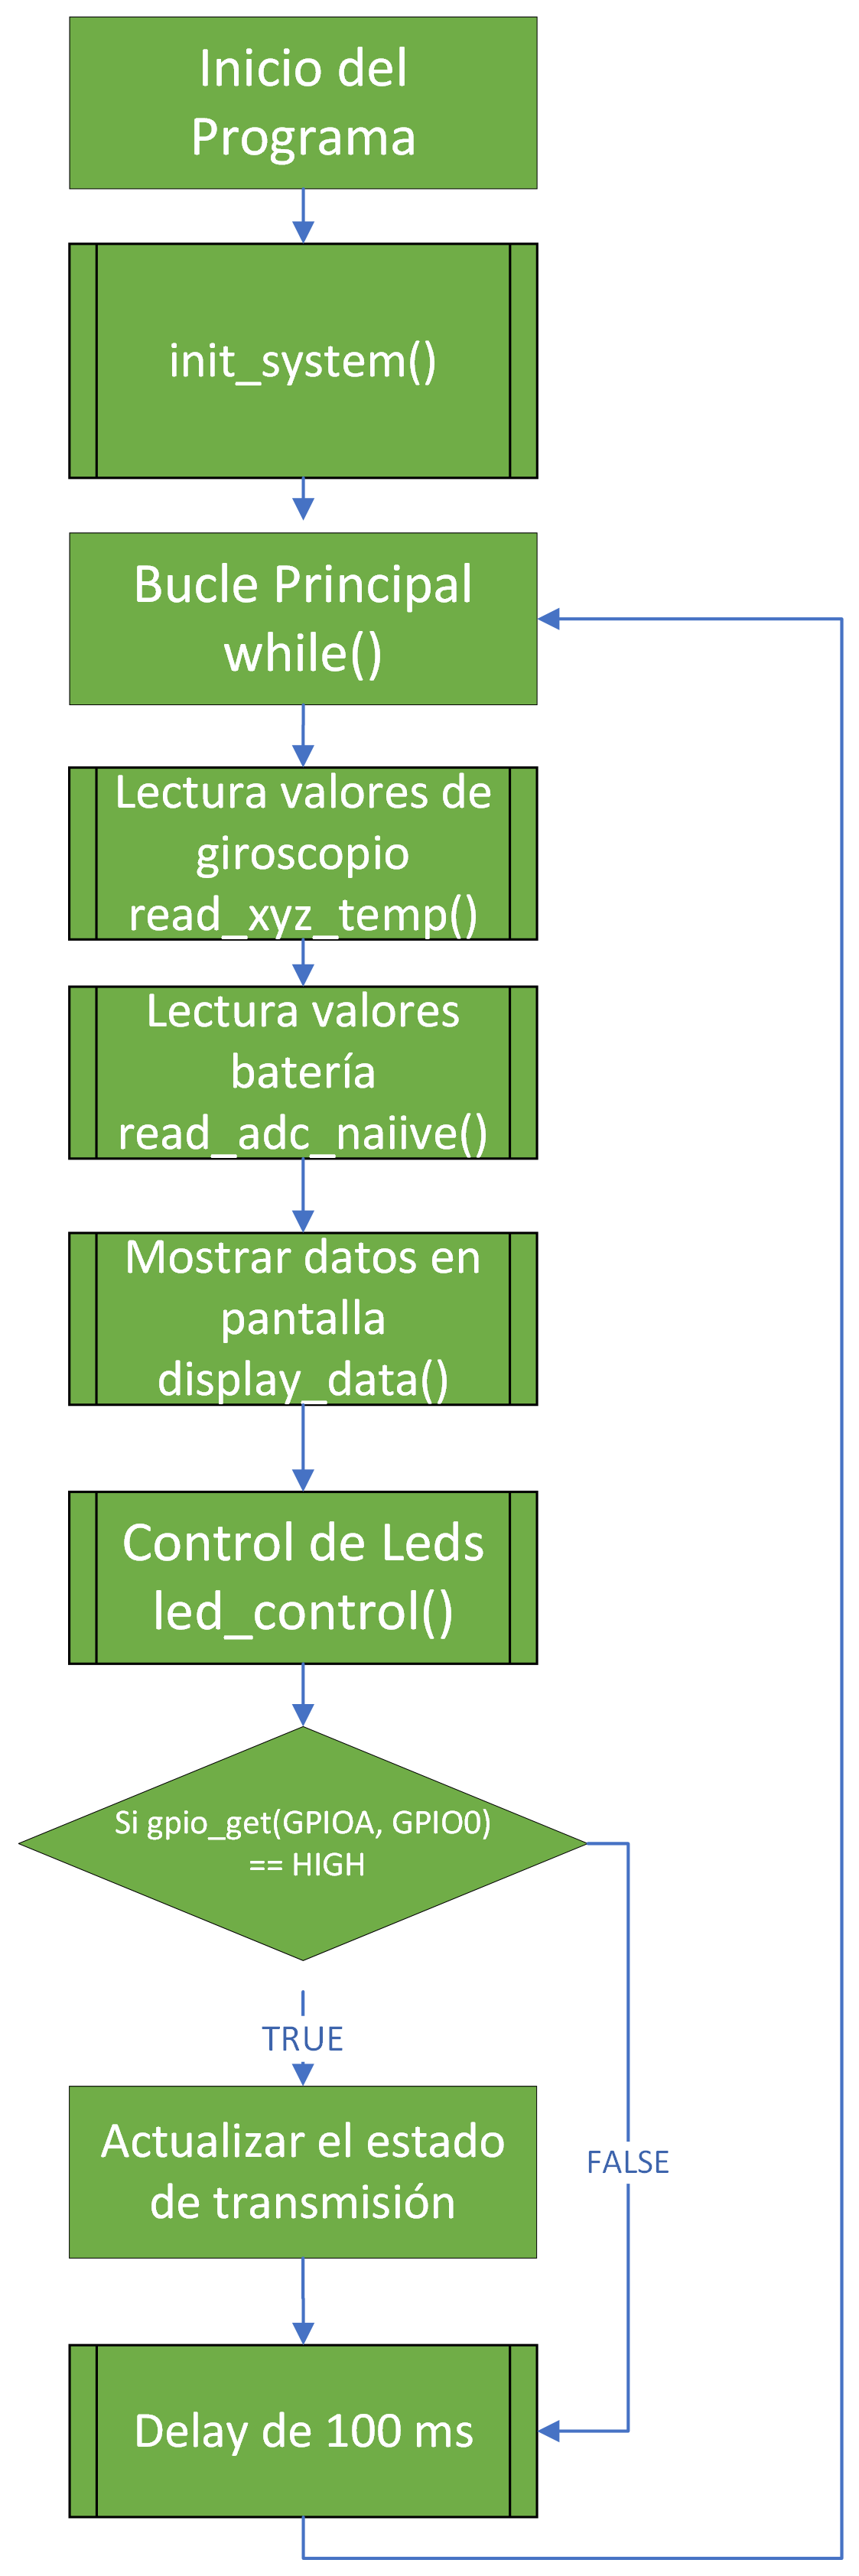
\includegraphics[scale = 0.58]{./Figuras/Desarrollo_Analisis/Diagrama_pendientes.png}
        \caption{Diagrama de flujo que describe el funcionamiento del sistema.}
    \end{figure}
\newpage

\subsubsection{\textit{Script} de Python \texttt{iot.py}}
Este \textit{script} en Python establece una comunicación serial el STM32F429 y utiliza MQTT para enviar los datos leídos a un \textit{broker}. Primero, configura la comunicación serial y el cliente MQTT, definiendo las funciones de conexión y los parámetros necesarios. Luego, verifica continuamente la conexión al broker MQTT y, una vez establecida, entra en un bucle donde lee datos del dispositivo, procesa estos datos (incluyendo detección de batería baja y deformación), los convierte a formato JSON, y los publica en el tema MQTT especificado. Este proceso se ejecuta indefinidamente, asegurando una transmisión continua de los datos a la plataforma Thingsboard.

\subsubsection{Construcción del circuito utilizado}
Para iniciar con la construcción de este circuito, es necesario tomar en cuenta el métodos de protección de tensión descrito en la sección \ref{sec:cir1}. Dado lo anterior, se toma como tensión de entrada la tensión entre la parte superior del resistor $R_{2}$. Como según el enunciado es necesario hacer una medición de tensión de la batería, el pin 3 del puerto A se conecta a la parte superior del resistor $R_{2}$ y el pin GND se conecta a la tierra del circuito. Por otro lado, para notificar una tensión baja (menor a 7 V), se utilizó el pin 14 del puerto G como salida, el cual corresponde a uno de los LED integrados, este parpadea cuando ocurre el caso mencionado. Asimismo, para notificar una deformación en el terreo, se utilizó el pin 13 de puerto G como salida, el cual corresponde a uno de los LED integrados, este también parpadea cuando ocurre el caso mencionado. Por otro lado, se utilizó el pin 0 del puerto A, el cual se configuró como entrega, ya que esta asociado al pulsador azul integrado, este permite seleccionar si la transmisión está o no habilitada. Finalmente, se utilizó la pantalla LCD del microcontrolador para desplegar los datos de tensión disponible en la batería, las velocidades angulares de cada eje, la temperatura y el estado de la transmisión de datos hacia Thingsboard. El circuito resultante tras implementar todas as consideraciones anteriores puede consultarse en la Figura \ref{fig:final}:

\begin{figure}[H]
\centering
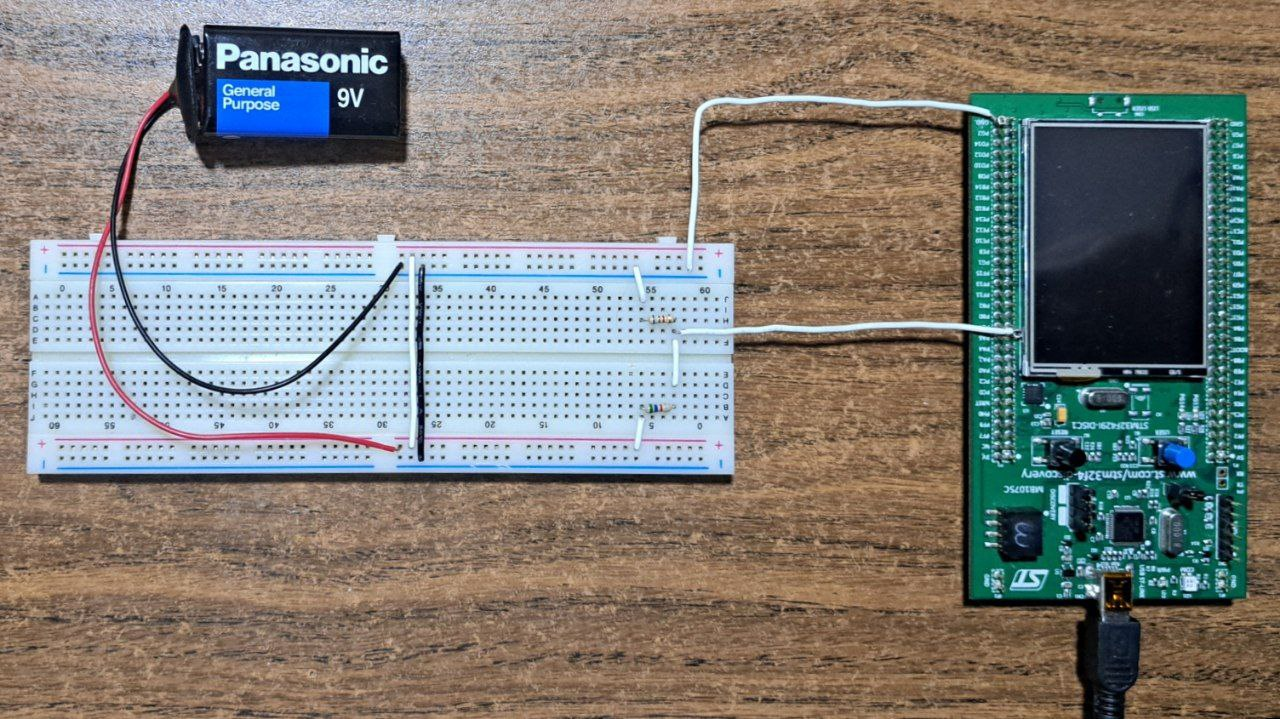
\includegraphics[width=125mm]{./Figuras/Desarrollo_Analisis/SYS}
\caption{Circuito final tras los cálculos de magnitudes y la implementación de las consideraciones necesarias.} 
\label{fig:final}
\end{figure}

\subsection{Análisis de los resultados}
 A continuación se mostrarán los resultados para cada una de las funcionalidades solicitadas por el enunciado: 

\subsubsection{Tensión de entrada adecuada}
En la Figura \ref{fig:5V} puede observarse la medida de tensión en $R_{2}$:

\begin{figure}[H]
\centering
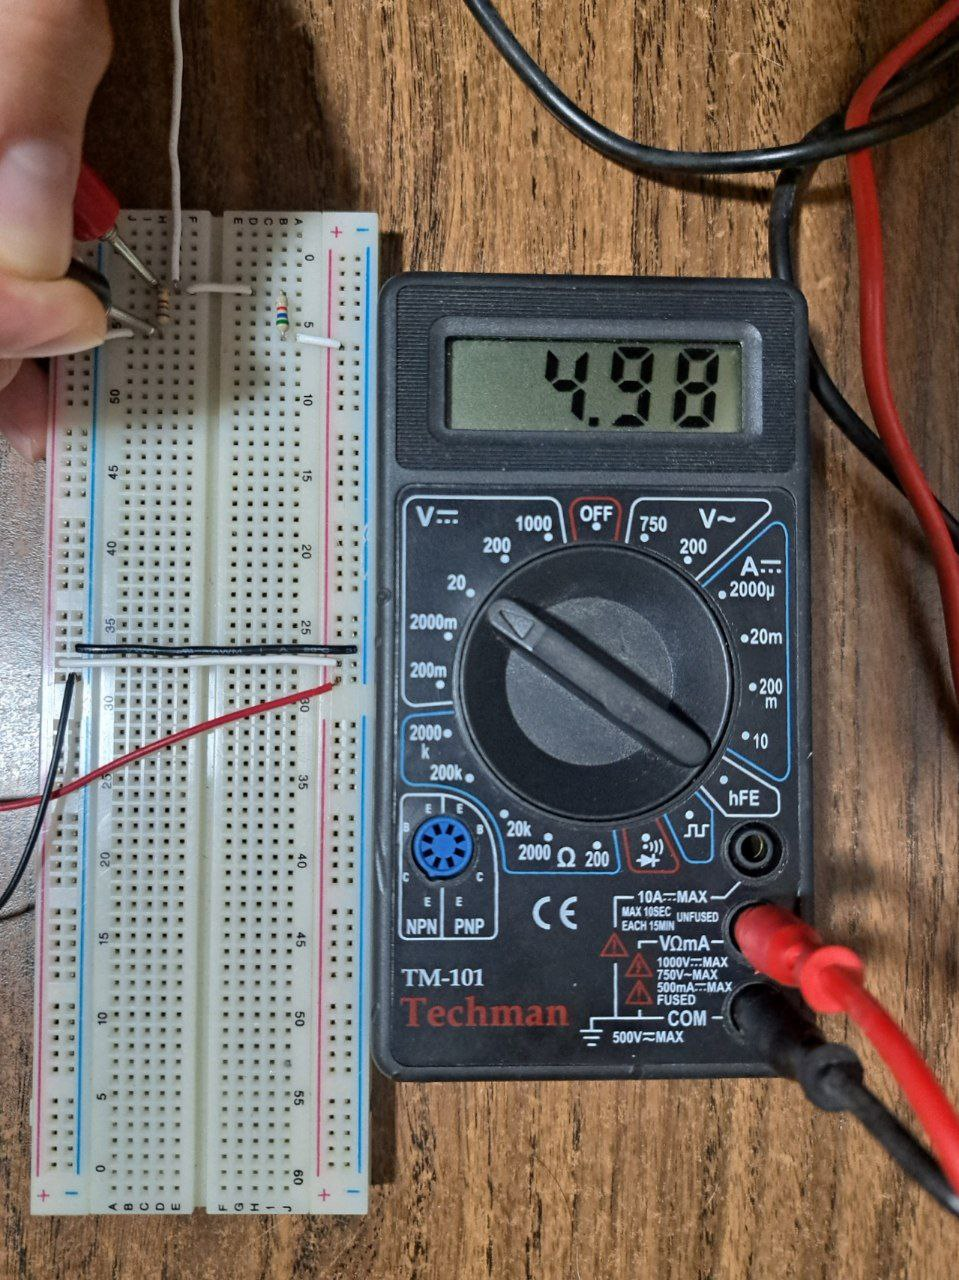
\includegraphics[width=80mm]{./Figuras/Desarrollo_Analisis/5V}
\caption{Tensión de entrada adecuada, la cual permitirá evaluar la tensión restante en la batería.} 
\label{fig:5V}
\end{figure}

Como puede verse en la Figura \ref{fig:5V}, la tensión de entrada es un valor cercano a los 5 V, tal como fue calculado en la sección \ref{sec:cir1}. Lo anterior permite que al microcontrolador entre una tensión adecuada y que se pueda hacer la evaluación de la tensión restante en la batería. 

\subsubsection{Despliegue de información en el microcontrolador}
En la Figura \ref{fig:STMa} puede observarse la información mostrada en el microcontrolador una vez que el programa fue cargado en este y la batería fue conectada:

\begin{figure}[H]
\centering
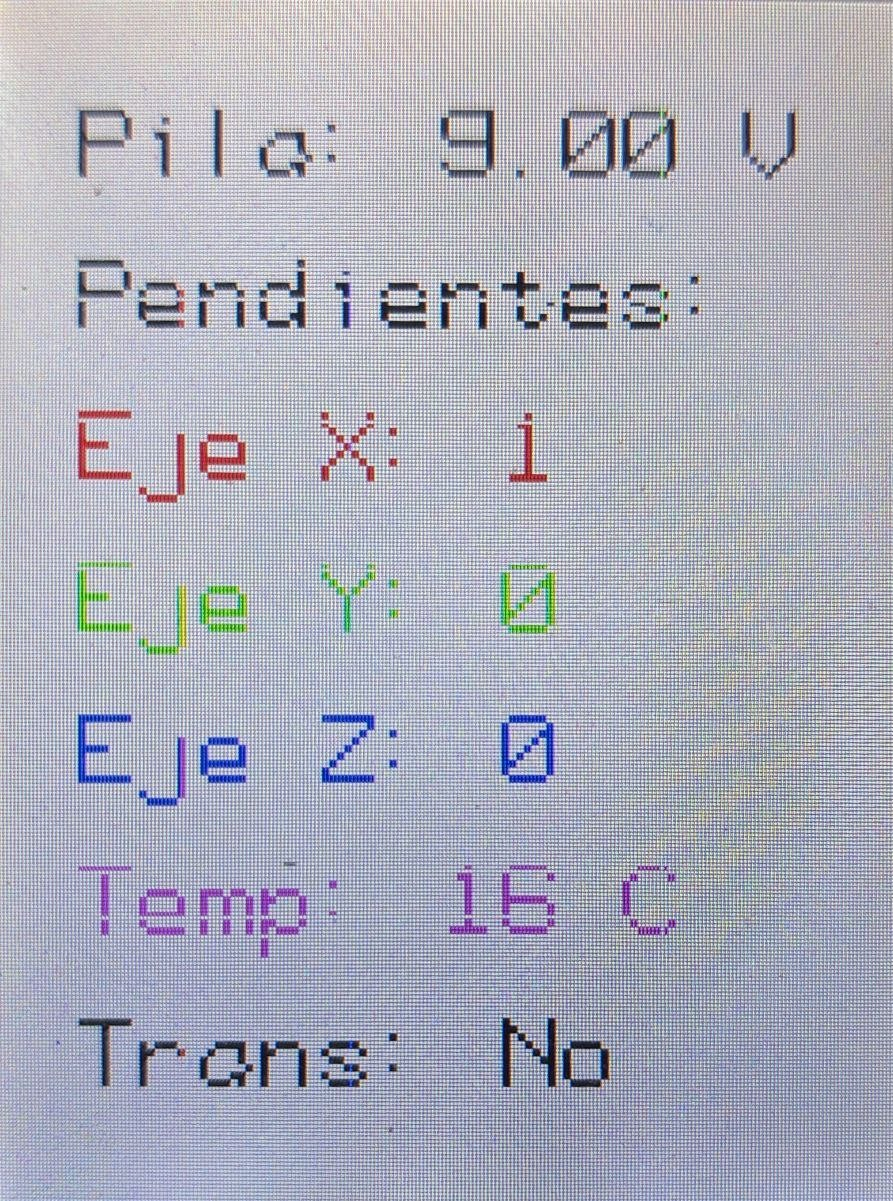
\includegraphics[width=55mm]{./Figuras/Desarrollo_Analisis/STMa}
\caption{Información desplegada en la pantalla al iniciar el sistema.} 
\label{fig:STMa}
\end{figure}

Como puede verse en la Figura \ref{fig:STMa}, en la pantalla efectivamente puede verse el valor de tensión de la batería (``Pila''), el valor de cada uno de los ejes (``Pendientes''), el valor de temperatura (``Temp'') y el estado de la transmisión (``Trans''). El valor de la temperatura no alcanza el valor correcto y esto se debe a que el sensor de temperatura del L3GD20 está destinado a compensar la variación del chip y no a medir la temperatura ambiental, además no se especifica un punto de referencia claro para el valor del offset en la hoja del fabricante, tal como se detalla en \cite{ADA}. A pesar de esto, lo anterior confirma que la programación realizada para extraer datos del acelerómetro fue exitosa y que el circuito para regular la entrada de tensión funciona correctamente.  

En la Figura \ref{fig:STMb}, puede observarse el resultado en pantalla cuando el botón de usuario es presionado: 

\begin{figure}[H]
\centering
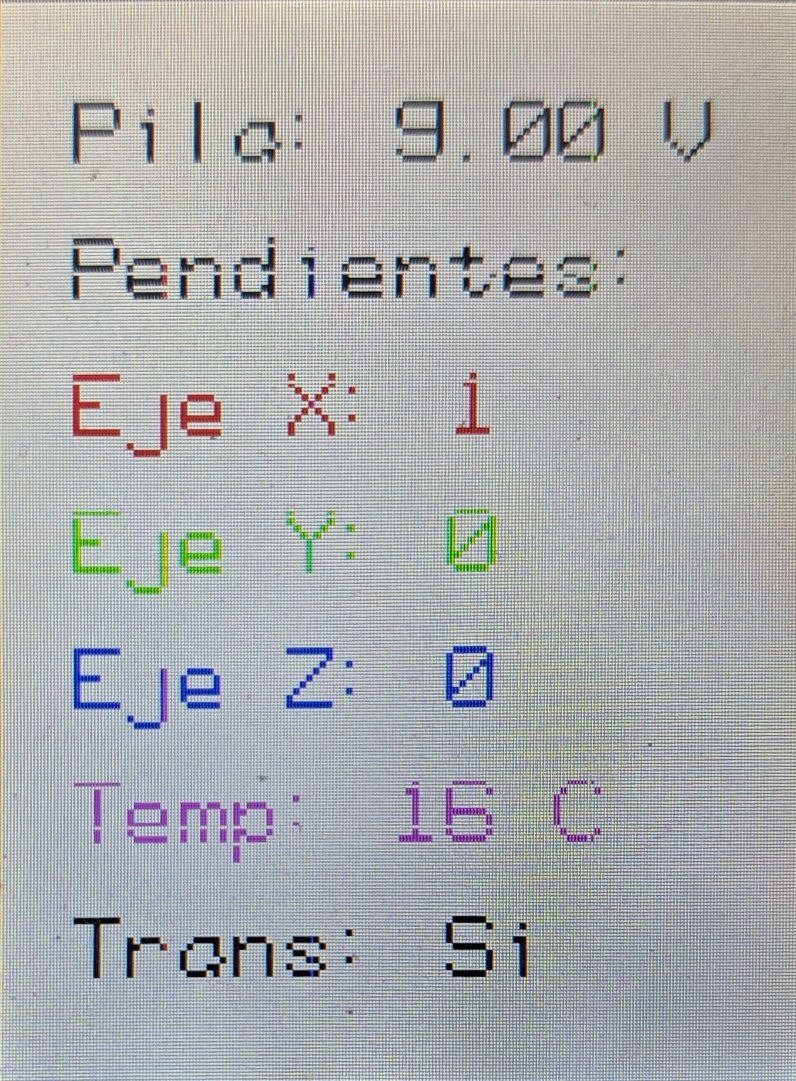
\includegraphics[width=55mm]{./Figuras/Desarrollo_Analisis/STMb}
\caption{Información desplegada en la pantalla cuando el botón de usuario fue presionado para habilitar la transmisión.} 
\label{fig:STMb}
\end{figure}

Como puede verse en la Figura \ref{fig:STMb}, la opción ``Trans'' pasó de estar en ``No'' a estar en ``Si'', confirmando que el botón para habilitar la transmisión funciona de manera correcta. Los resultados obtenidos en la plataforma de IoT puede consultarse en la siguiente sección. 

Por último, para demostrar el funcionamiento de los LED que funciona como banderas para notificar que cambios en la pendiente del terreno en el que se encuentra el sisema y que la batería está baja, pueden consultarse en el siguiente video: \url{https://youtu.be/xIwpAetdkUw}. En este pueden observarse tres estados: 

\begin{enumerate}
    \item Al inicio del video puede observarse como ninguno de los LED parpadean, ya que la batería está conectada y cuenta con un valor adecuado. 

    \item El LED verde parpadea cuando ocurre un cambio de la pendiente que es superior a 5 grados. Asimismo, se pueden notar los cambios en la velocidad angular de los ejes. 

    \item El LED rojo parpadea cuando se desconecta la batería, indicando un valor inferior a 7 V. También puede verse como la tensión baja en la pantalla y como cambia debido al ruido de lectura en el pin. 
\end{enumerate}

Estos tres estados confirman la notificación adecuada de incidentes utilizando la información ambiental, para cada uno de los casos solicitados en el enunciado. Al igual que con los resultados de transmisión, los casos anteriores podrán verse reflejados en la siguiente sección. 

\subsubsection{Transmisión de datos a Thingsboard}

Para el despliegue de datos, se utilizó la plataforma Thingsboard. Con el sistema conectado, el programa cargado en el microcontrolador, la transmisión habilitada y el identificador del dispositivo configurado en la plataforma, se corre el \texttt{script} Python. Al correr el \textit{script}, se evalúa la conexión y una vez que se logra, se imprime ``Conexión exitosa.'' en la terminal. Ya con la conexión establecida, se obtiene el siguiente resultado en la terminal, el cual puede ser observado en la Figura \ref{fig:CONE}: 

\begin{figure}[H]
\centering
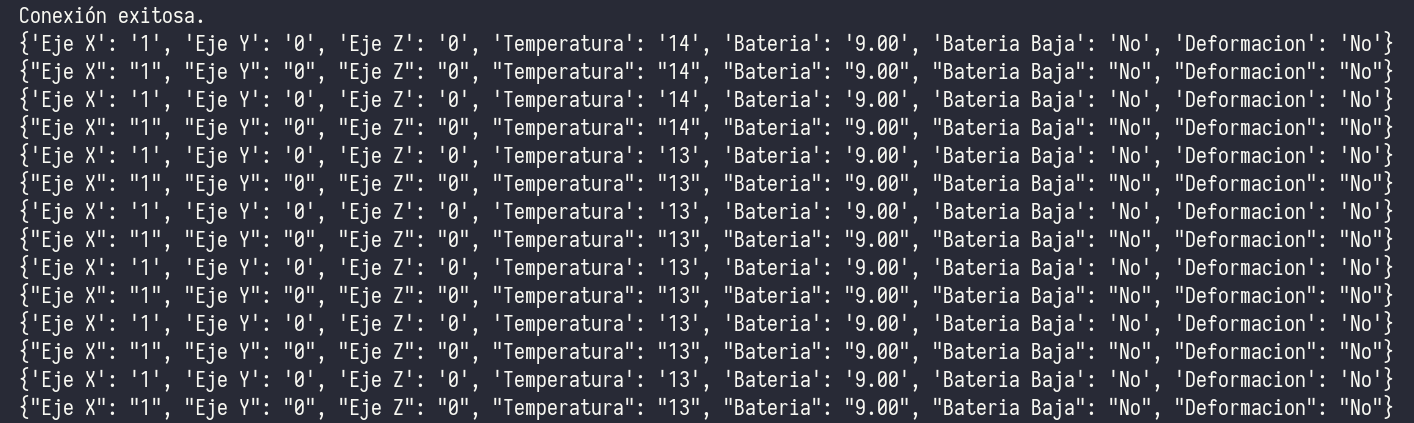
\includegraphics[width=155mm]{./Figuras/Desarrollo_Analisis/CONE}
\caption{Transmisión de datos Thingsboard utilizando el \texttt{script} de Python.} 
\label{fig:CONE}
\end{figure}

Como puede verse en la Figura \ref{fig:CONE}, los datos relevantes del sistema son transmitidos a la plataforma de IoT. Estos fueron utilizados para la construcción de un \textit{dashboard} que permite visualizar de manera más accesible los datos y controlar las alertas de casos de interés. Dicho \textit{dashboard} puede consultarse en el siguiente link: \href{https://iot.eie.ucr.ac.cr/dashboard/dfa4a2d0-184a-11ef-b343-e18dce159afc?publicId=f5fe9880-9148-11ee-9eb1-4f281083cad4}{Slope Monitoring Dashboard}. Asimismo, este puede observarse en la Figura \ref{fig:DSBD}: 

\begin{figure}[H]
\centering
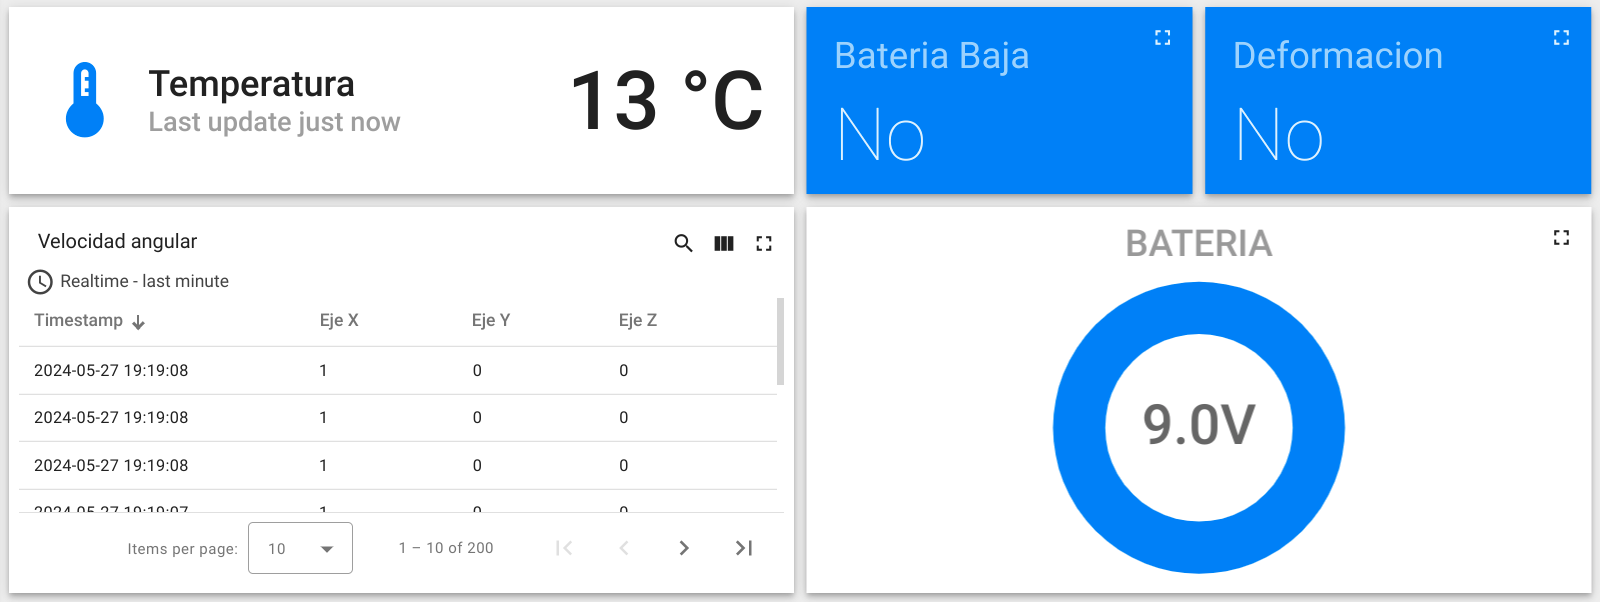
\includegraphics[width=155mm]{./Figuras/Desarrollo_Analisis/DSBD}
\caption{\textit{Dashboard} construido en Thingsboard para monitorear el sistema de monitoreo de cambios en la pendiente de un terreno.} 
\label{fig:DSBD}
\end{figure}

Como puede verse en la Figura \ref{fig:DSBD}, en este se muestran los datos de los tres ejes del acelerómetro, la temperatura, la información sobre la carga de la batería y las dos notificaciones que muestran si la batería tiene un carga menor a 7 V y si hubo una deformación en el terreno. 

Finalmente, pueden observarse los tres casos de estado descritos en la sección anterior: 

\begin{enumerate}
    \item El \textit{dashboard} tiene datos estáticos, ya que no hay cambios de pendiente y la batería se encuentra en su carga óptima. Lo anterior puede consultarse en la Figura \ref{fig:DSBD}.

    \item Se notifica una deformación en el terreno de más de 5 grados. Asimismo, se pueden notar los cambios en la velocidad angular de los ejes. Lo anterior puede consultarse en la Figura \ref{fig:TH2}: 

    \begin{figure}[H]
    \centering
    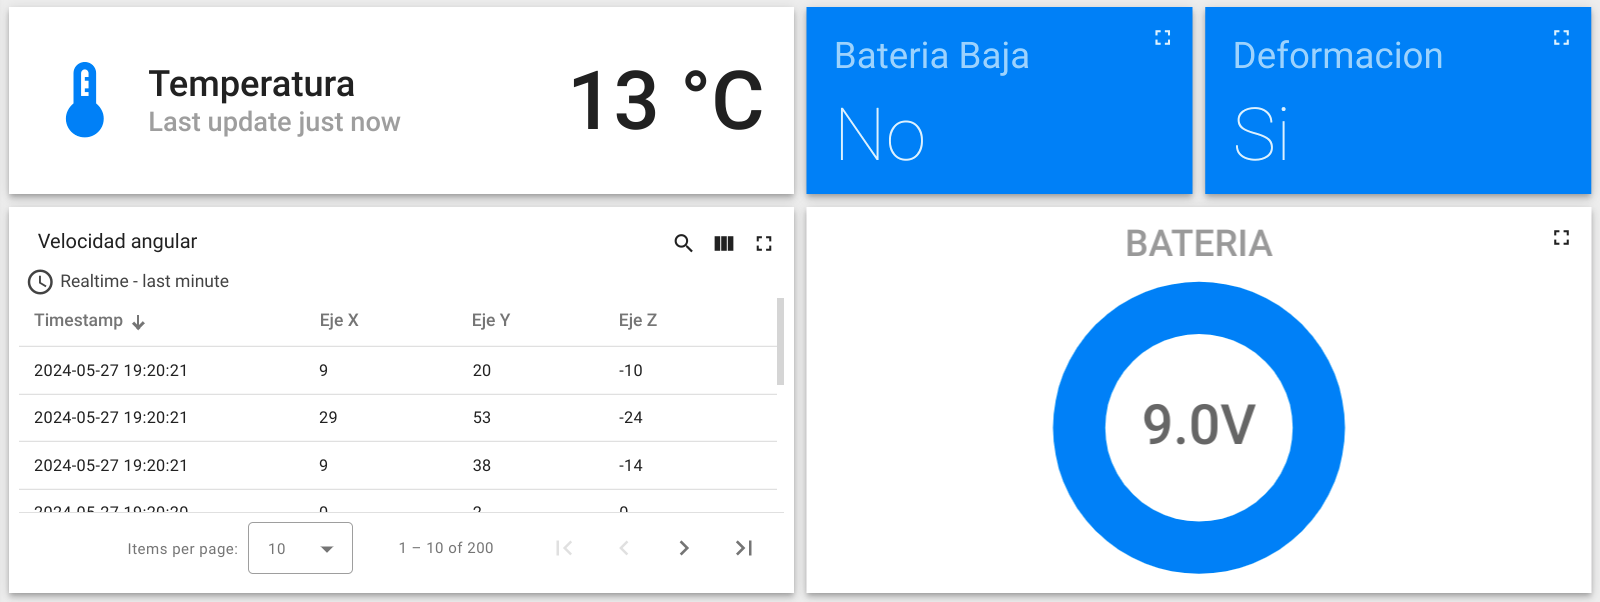
\includegraphics[width=155mm]{./Figuras/Desarrollo_Analisis/TH2}
    \caption{Comportamiento del \textit{dashboard} tras un cambio en la pendiente del terreno en el que se encuentra el sistema.} 
    \label{fig:TH2}
    \end{figure}

    \item Se notifica que la batería tiene una carga inferior a 7 V. Lo anterior también se puede notar en la métrica encargada de la carga de batería. Lo anterior puede consultarse en la Figura \ref{fig:TH3}: 

    \begin{figure}[H]
    \centering
    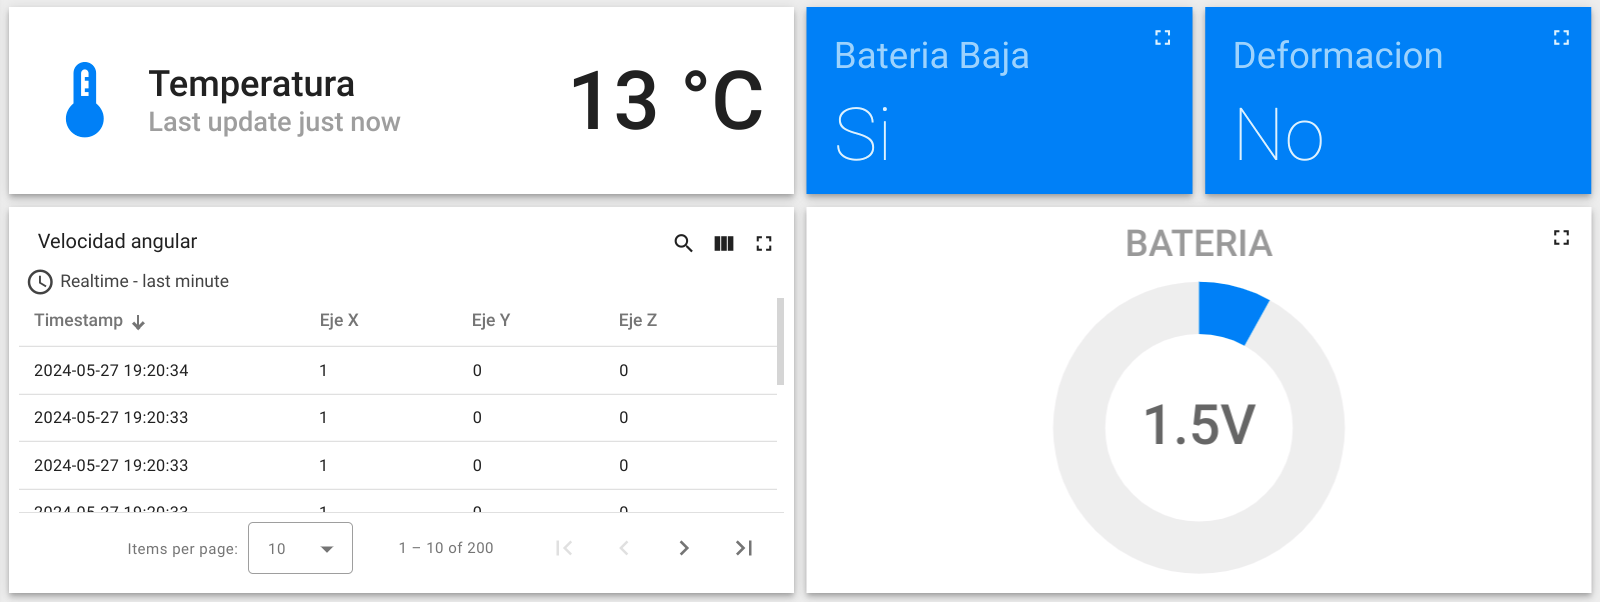
\includegraphics[width=155mm]{./Figuras/Desarrollo_Analisis/TH3}
    \caption{Comportamiento del \textit{dashboard} tras una disminución de la carga de la batería por debajo del umbral de tensión requerido.} 
    \label{fig:TH3}
    \end{figure}
\end{enumerate}

Estos tres estados confirman la notificación adecuada de incidentes utilizando la información extraída del microcontrolador y enviada a la plataforma de IoT, confirmando el cumplimiento de los objetivos del laboratorio, detallados en el enunciado.  